\section*{Anhang}
\addcontentsline{toc}{section}{Anhang}
\label{sec:anhang}
 
 % Table generated by Excel2LaTeX from sheet 'Daten'
 \begin{table}[h!]
 	\renewcommand*{\arraystretch}{1.2}
 	\centering
 	\caption{Analytdaten bei $\lambda_{1}$ für Permanganat-Ionen ohne Querempfindlichkeiten}
 	\label{tab:stat_oQ_m}	
 	\resizebox{16.cm}{!}{
 			\begin{tabulary}{1.8\textwidth}{C|CCC|C|C|C|C|C|C}
 				\hline
 				\textbf{\SI{525}{\nano \meter}} & \textbf{$c_1 \, \left[\si{\milli \mol \per \liter}\right]$} & \textbf{$c_2 \, \left[\si{\milli \mol \per \liter}\right]$} & \textbf{$c_3 \, \left[\si{\milli \mol \per \liter}\right]$} &\textbf{MW $\left[\si{\milli \mol \per \liter}\right]$} & \textbf{Wahrer W. }$\left[\si{\milli \mol \per \liter}\right]$& \textbf{Fehler} $\left[\si{\percent}\right]$ & \textbf{$s \, \left[\si{\milli \mol \per \liter}\right]$} &  $N$ & \textbf{conf} $\left[\pm \si{\milli \mol \per \liter}\right]$\\
 				\hline
 				A1 & 0,2234&0,2235&0,2234&0,2234&0,2130&4,9&\SI{9,22e-5}{}&3&\SI{2,29e-4}{}\\
 				A2 & 0,1517&0,1517&0,1517&0,1517&0,20&-24,1&\SI{3,80e-5}{}&3&\SI{9,44e-5}{}\\
 				\hline
 	\end{tabulary}
 }
 \end{table}%
 \FloatBarrier
 
 % Table generated by Excel2LaTeX from sheet 'Daten'
 \begin{table}[h!]
 	\renewcommand*{\arraystretch}{1.2}
 	\centering
 	\caption{Analytdaten bei $\lambda_{2}$ für Dichromat-Ionen ohne Querempfindlichkeiten}
 	\label{tab:stat_oQ_c}	
 	\resizebox{16.cm}{!}{
 		\begin{tabulary}{1.8\textwidth}{C|CCC|C|C|C|C|C|C}
 			\hline
 			\textbf{\SI{352}{\nano \meter}} & \textbf{$c_1 \, \left[\si{\milli \mol \per \liter}\right]$} & \textbf{$c_2 \, \left[\si{\milli \mol \per \liter}\right]$} & \textbf{$c_3 \, \left[\si{\milli \mol \per \liter}\right]$} &\textbf{MW $\left[\si{\milli \mol \per \liter}\right]$} & \textbf{Wahrer W. }$\left[\si{\milli \mol \per \liter}\right]$& \textbf{Fehler} $\left[\si{\percent}\right]$ & \textbf{$s \, \left[\si{\milli \mol \per \liter}\right]$} &  $N$ & \textbf{conf} $\left[\pm \si{\milli \mol \per \liter}\right]$\\
 			\hline
 			A1 & 0,1918&0,1919&0,1922&0,1920&0,10&92,0&\SI{2,16e-4}{}&3&\SI{5,36e-4}{}\\
 			A2 & 0,2358&0,2358&0,2358&0,2358&0,15&57,2&\SI{1,90e-5}{}&3&\SI{4,72e-5}{}\\
 			\hline
 		\end{tabulary}
 	}
 \end{table}%
 \FloatBarrier
 
  % Table generated by Excel2LaTeX from sheet 'Daten'
 \begin{table}[h!]
 	\renewcommand*{\arraystretch}{1.2}
 	\centering
 	\caption{Analytdaten bei $\lambda_{1}$ für Permanganat-Ionen mit Querempfindlichkeiten}
 	\label{tab:stat_mQ_m}	
 	\resizebox{16.cm}{!}{
 		\begin{tabulary}{1.8\textwidth}{C|CCC|C|C|C|C|C|C}
 			\hline
 			\textbf{\SI{525}{\nano \meter}} & \textbf{$c_1 \, \left[\si{\milli \mol \per \liter}\right]$} & \textbf{$c_2 \, \left[\si{\milli \mol \per \liter}\right]$} & \textbf{$c_3 \, \left[\si{\milli \mol \per \liter}\right]$} &\textbf{MW $\left[\si{\milli \mol \per \liter}\right]$} & \textbf{Wahrer W. }$\left[\si{\milli \mol \per \liter}\right]$& \textbf{Fehler} $\left[\si{\percent}\right]$ & \textbf{$s \, \left[\si{\milli \mol \per \liter}\right]$} &  $N$ & \textbf{conf} $\left[\pm \si{\milli \mol \per \liter}\right]$\\
 			\hline
 			A1 & 0,2205&0,2207&0,2205&0,2205&0,213&3,5&\SI{9,04e-5}{}&3&\SI{2,24e-4}{}\\
 			A2 & 0,2070&0,2070&0,2069&0,2070&0,20&3,5&\SI{5,02e-5}{}&3&\SI{1,25e-4}{}\\
 			\hline
 		\end{tabulary}
 	}
 \end{table}%
 \FloatBarrier
 
  % Table generated by Excel2LaTeX from sheet 'Daten'
 \begin{table}[h!]
 	\renewcommand*{\arraystretch}{1.2}
 	\centering
 	\caption{Analytdaten bei $\lambda_{2}$ für Dichromat-Ionen mit Querempfindlichkeiten}
 	\label{tab:stat_mQ_c}	
 	\resizebox{16.cm}{!}{
 		\begin{tabulary}{1.8\textwidth}{C|CCC|C|C|C|C|C|C}
 			\hline
 			\textbf{\SI{352}{\nano \meter}} & \textbf{$c_1 \, \left[\si{\milli \mol \per \liter}\right]$} & \textbf{$c_2 \, \left[\si{\milli \mol \per \liter}\right]$} & \textbf{$c_3 \, \left[\si{\milli \mol \per \liter}\right]$} &\textbf{MW $\left[\si{\milli \mol \per \liter}\right]$} & \textbf{Wahrer W. }$\left[\si{\milli \mol \per \liter}\right]$& \textbf{Fehler} $\left[\si{\percent}\right]$ & \textbf{$s \, \left[\si{\milli \mol \per \liter}\right]$} &  $N$ & \textbf{conf} $\left[\pm \si{\milli \mol \per \liter}\right]$\\
 			\hline
 			A1 & 0,1099&0,1099&0,1103&0,1100&0,10&10,0&\SI{2,10e-4}{}&3&\SI{5,22e-4}{}\\
 			A2 & 0,1579&0,1579&0,1579&0,1579&0,15&5,3&\SI{5,77e-7}{}&3&\SI{1,43e-6}{}\\
 			\hline
 		\end{tabulary}
 	}
 \end{table}%
 \FloatBarrier
 
 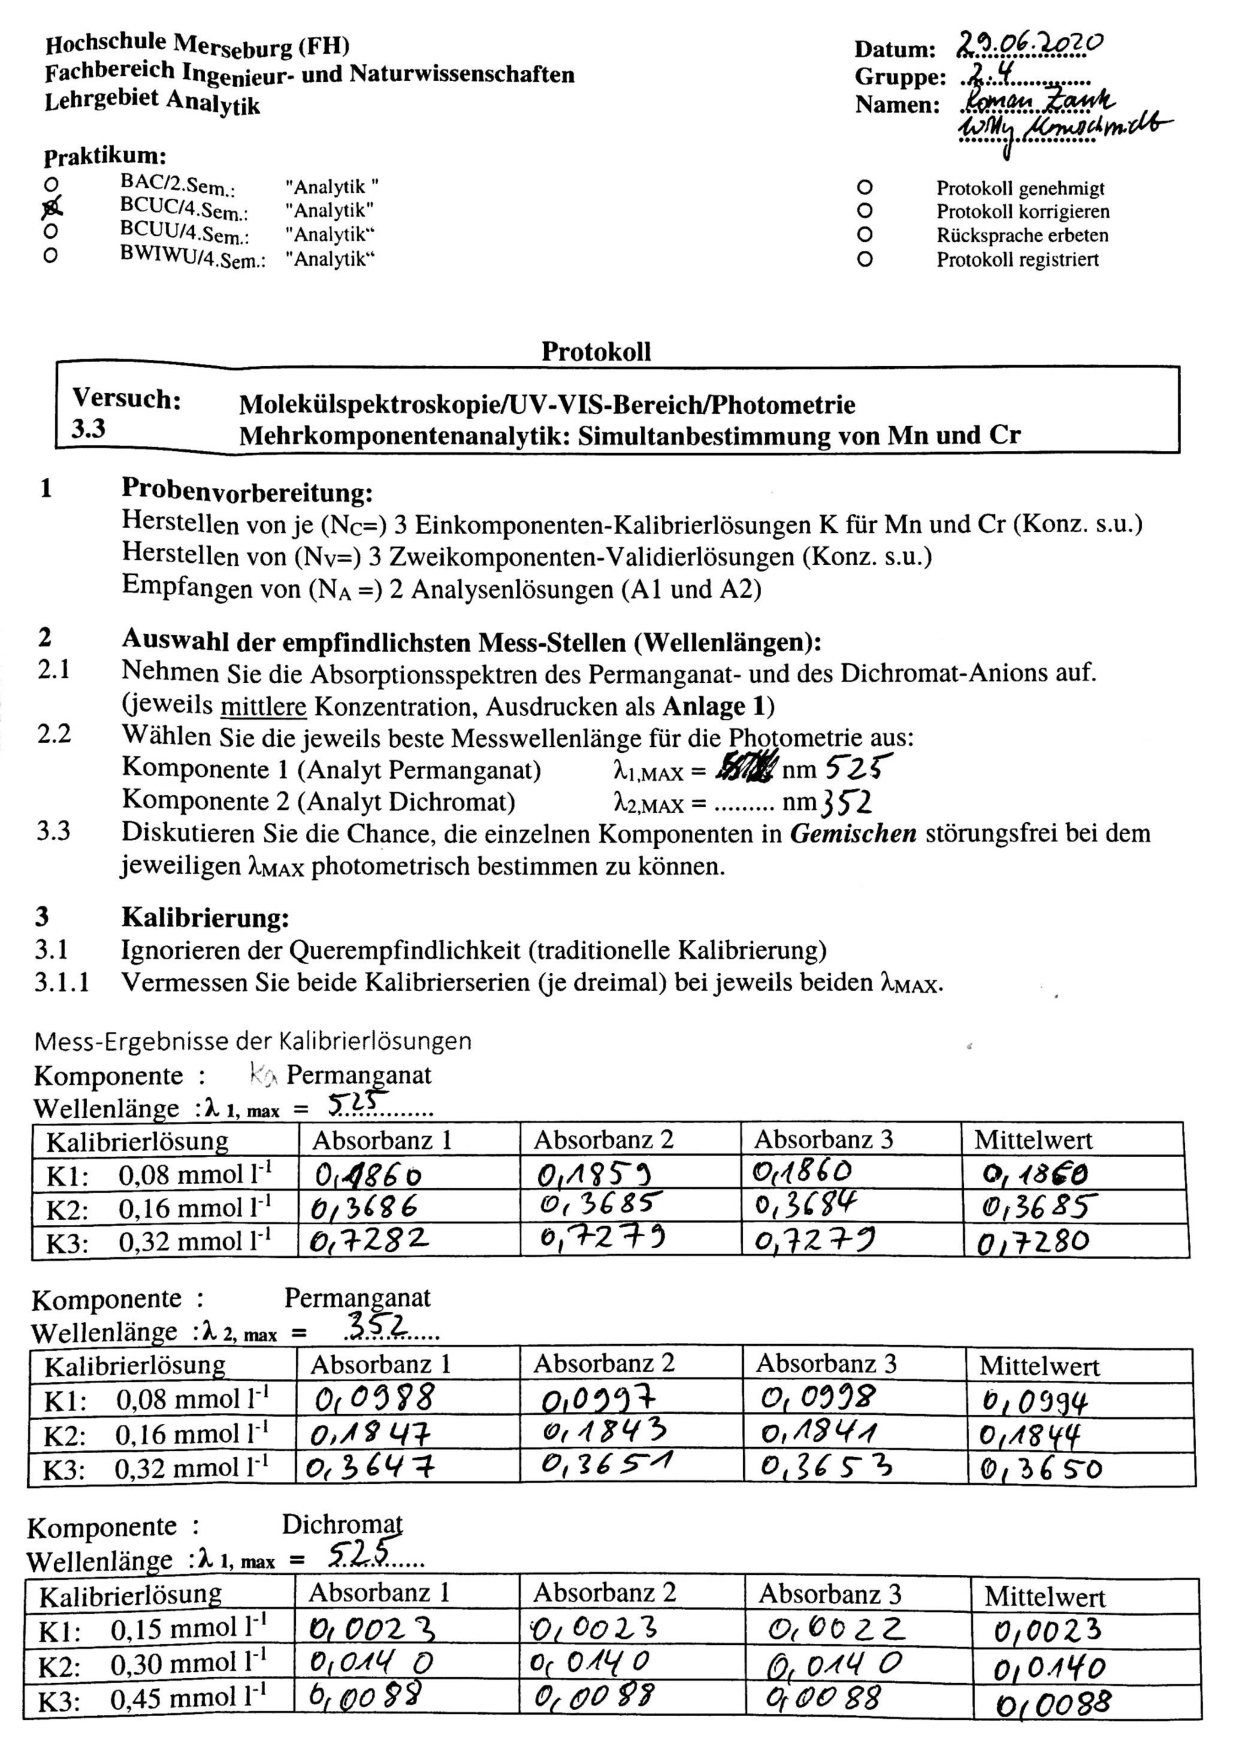
\includepdf[pages=1-3]{data/data_v33.pdf}
 